\begin{sidewaysfigure}
	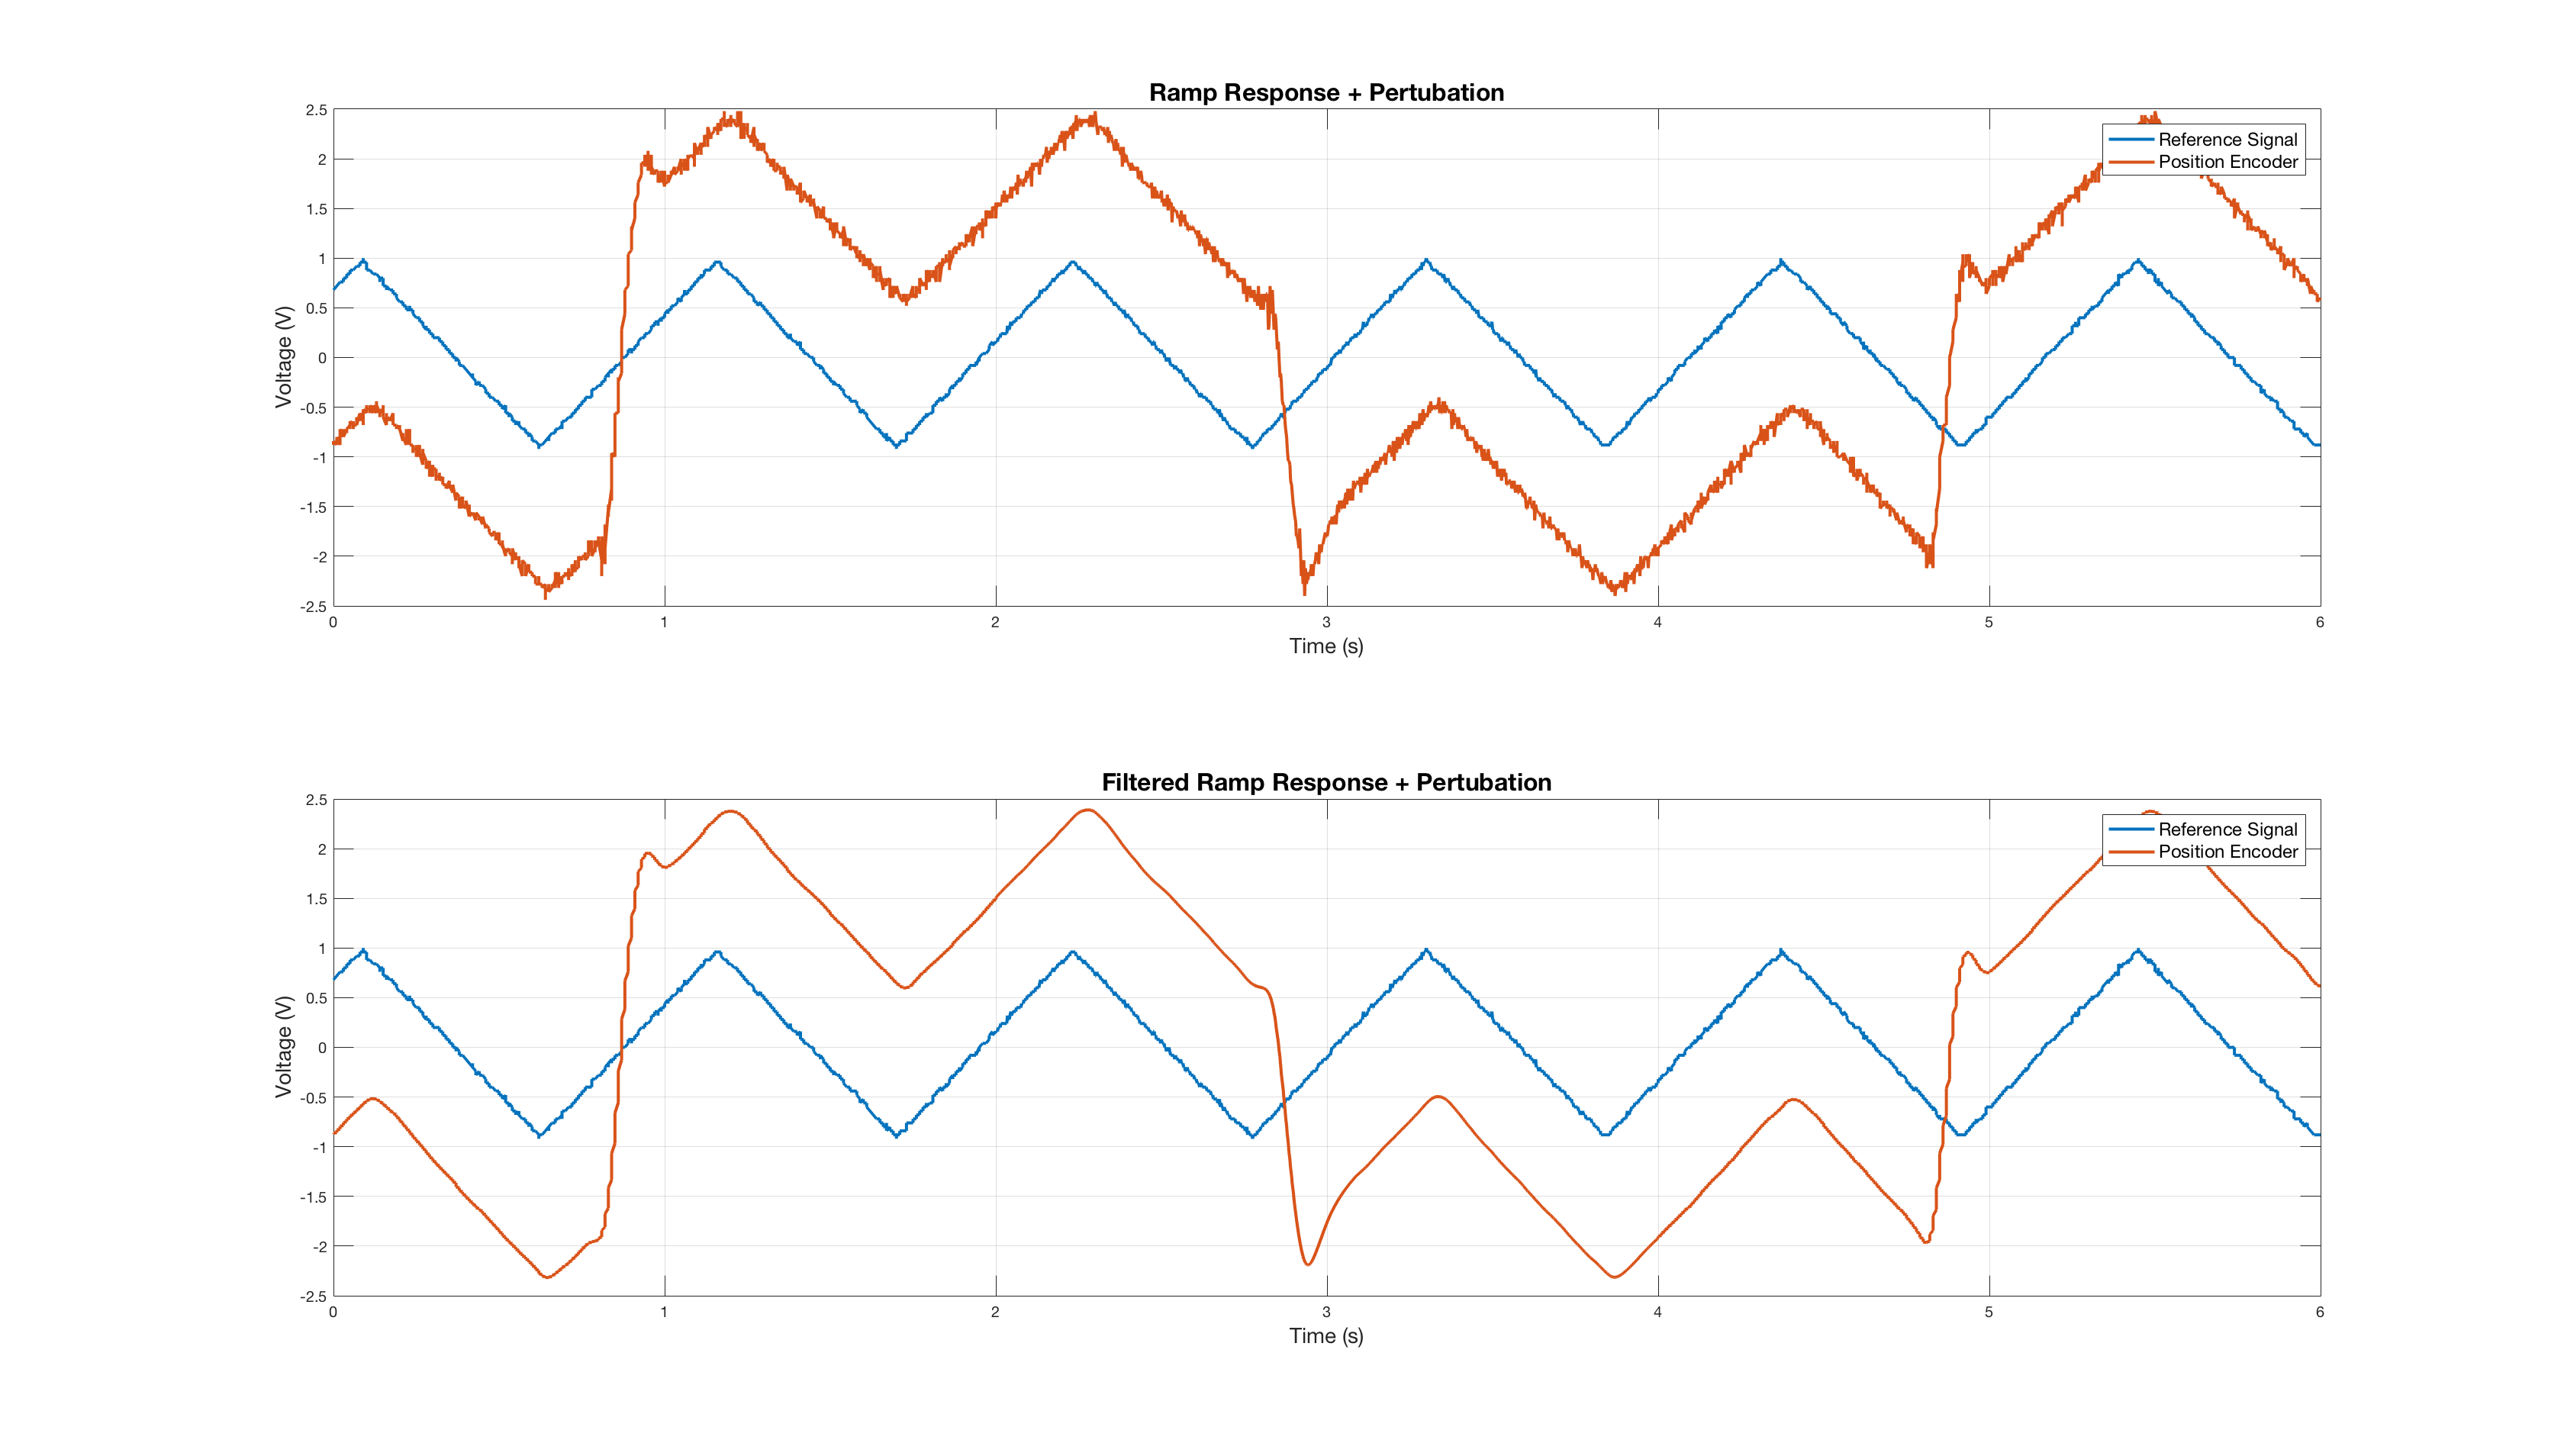
\includegraphics[width=\textheight]{img/results/ramp_noise.png}
    \caption{Resposta do sistema à entrada rampa unitária com pertubação de onda quadrada de $0.25 Hz$ e $2V$ pico a pico. Estão representados tanto o sinal original lido no osciloscópio, como um sinal filtrado para remover ruídos de alta frequência. O ponto utilizado para medição do erro em regime permanente foi $time=0.5s$}
    \label{fig::ramp_noise_response}
\end{sidewaysfigure}
